\documentclass[c]{beamer}
\usepackage[beamer, logo=bibi, fr, maths, tensoriel]{jd}
%\usepackage{asymptote}

\hypersetup{%
  pdftitle={Ondes internes de gravité},%
  pdfkeywords={igw, viscosity},%
}

\title[IGW, vents \& viscosité]{Ondes internes de gravité atmosphériques}
\subtitle{caractérisation de l'effets des vents et de la viscosité}
\institute[UPMC]{Université Pierre et Marie Curie\\ \vspace{2em}\includegraphics[width=0.1\paperwidth]{upmc}}


\begin{document}

\frame[plain]{\titlepage}
\frame[plain]{\tableofcontents}

% --------------------
\section{présentation}

\subsection{laboratoire d'accueil}

\begin{frame}
\frametitle{Ganymède}
Équipe \bleu{Études spatiales et planétologie} (IPGP)\\
Axes de recherche :
\begin{itemize}
    \item étude des \textbf{couplages Terre--océan--atmosphère} : « depuis les perturbations atmosphériques transitoires provoquées par les séismes et les tsunamis, jusqu'aux intéractions à long terme entre la dynamique interne et l'atmosphère des planètes » ;
    \item étude de la \textbf{structure et de la dynamique interne des planètes} : « depuis la structure profonde vue par la sismologie, jusqu'aux lithosphères planétaires vues par la gravimétrie, en passant par la modélisation numérique de la dynamique interne des planètes telluriques. »
\end{itemize}
\end{frame}

\subsection{les ondes internes de gravité}

\begin{frame}
\frametitle{principe}
Un milieu fluide, stratifié, soumis à une perturbation, met en jeu :
\begin{itemize}
    \item le forçage induisant la stratification (gravité…) ;
    \item une force de rappel liée à la stratification (force d'archimède…).\plop
\end{itemize}
Équations primitives : les ondes internes de gravité (IGW) représentent une classe de solutions assez large, de nombreux phénomènes sont représentables selon les approximations utilisées en fonction du milieu (océan, atmosphère et échelles d'étude).
\end{frame}

\begin{frame}
\frametitle{IGW atmosphériques}
\begin{itemize}
    \item \textbf{sources} : relief, nuages, turbulence…
    \item \textbf{propagation} : anisotrope (stratification), dispersive ou non
    \item \textbf{interactions} : transport d'énergie et de quantité de mouvement sous contrainte des phénomènes dissipatifs (flux de chaleur, viscosité…) et de couplage (ondes-ondes, ondes-flux moyen, turbulence…)\plop
\end{itemize}
Paramétrer finement la signature atmosphérique doit permettre de remonter aux caractéristiques sources.
% étude mono-paramétrique
\end{frame}

%\begin{frame}
%\frametitle{interactions atmosphériques}
%plus en détail, les phénomènes dissipatifs qu'on va étudier
%ce qu'en dit Fritts
%\end{frame}

%\begin{frame}
%\frametitle{couplage sismique}
%\end{frame}

% -------------------------
\section{effet des vents}

\subsection{le modèle physique}

\begin{frame}
\frametitle{théorie linéaire, perturbations}
\begin{subnumcases}{\label{eq:systeme}}
    \lp \delt{} + \vv \cdot \gradient \rp \vv &    $= -\frac{1}{\rho} \gradient P$    \label{eq:systeme-un} \notag \\
    \divergence \vv &                      $= 0$                                                \label{eq:systeme-deux} \notag \\
    \delt \rho + \divergence{\rho \vv} &   $= 0$                                                \label{eq:systeme-trois} \notag
\end{subnumcases}
\begin{itemize}
    \item décomposition : $X = X_0(z) + X_1(x,y,z,t)$ avec $X_1 \ll X_0$
    \item perturbation : $X_1(x,y,z,t) = \tilde X(z) \cdot {\mathrm e^{i(\overbrace{k_x x + k_y y - \omega t}^{\textrm{phase~} \Phi})}}$
    \item linéarisation au premier ordre
\end{itemize}
\end{frame}

\begin{frame}
\frametitle{propagation pseudo-spectrale}
\pifpaf{phase 2D en espace $\Rightarrow \dz V = A V$}
\begin{align}
V & =
\begin{pmatrix}
    \tuz^* \notag \\
    \tp^*  \notag
\end{pmatrix} \\
A & =
\begin{bmatrix}
    -\frac{1}{\Omega} \lp k_x \dz \uxc + k_y \dz \uyc \rp + \frac{1}{2} \dz{\ln{\rho_0}} & -\frac{i \lp k_x^2 + k_y^2 \rp}{\Omega}   \\
    i \lp \Omega + \frac{g}{\Omega} \dz{\ln{\rho_0}} \rp                                  & -\frac{1}{2} \dz{\ln{\rho_0}}             \notag
\end{bmatrix}
\end{align}
\end{frame}

\subsection{implémentation numérique, résultats}

%\begin{frame}
%\frametitle{?}
%\end{frame}

%\begin{frame}
%\frametitle{Stabilité}
%\end{frame}

\begin{frame}
\frametitle{l'effet de filtre directionnel}
%TODO figures : modes pour vent parallèle, perpendiculaire, complet, cas along et against propagation
\begin{figure}[!ht]
\centering
\subfigure[]{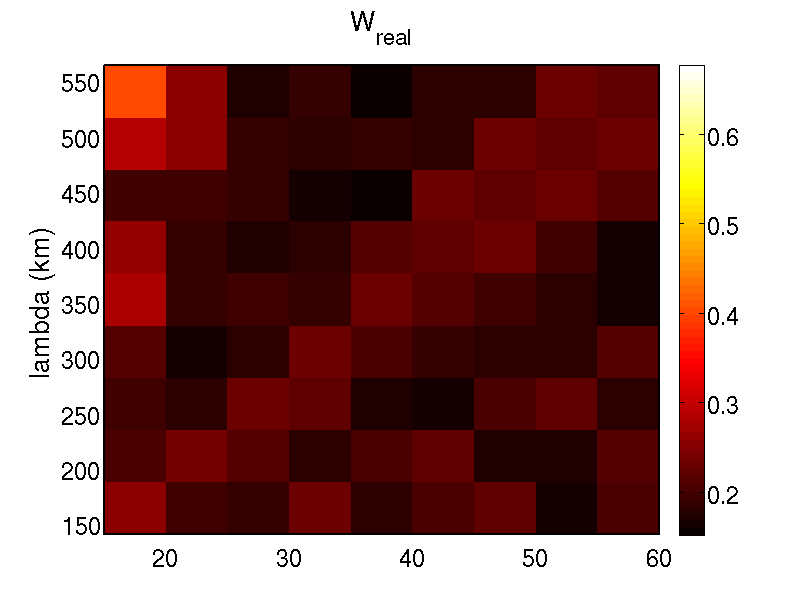
\includegraphics[width=0.4\linewidth]{scales_wM0Z0_T15-5-60_Lauto}}
\subfigure[]{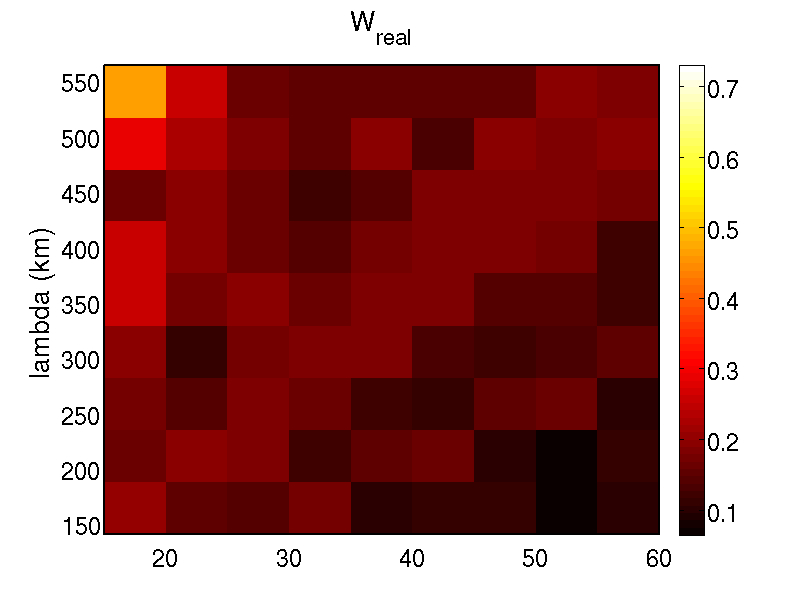
\includegraphics[width=0.4\linewidth]{scales_wMautoZ0_T15-5-60_Lauto}}\\
\subfigure[]{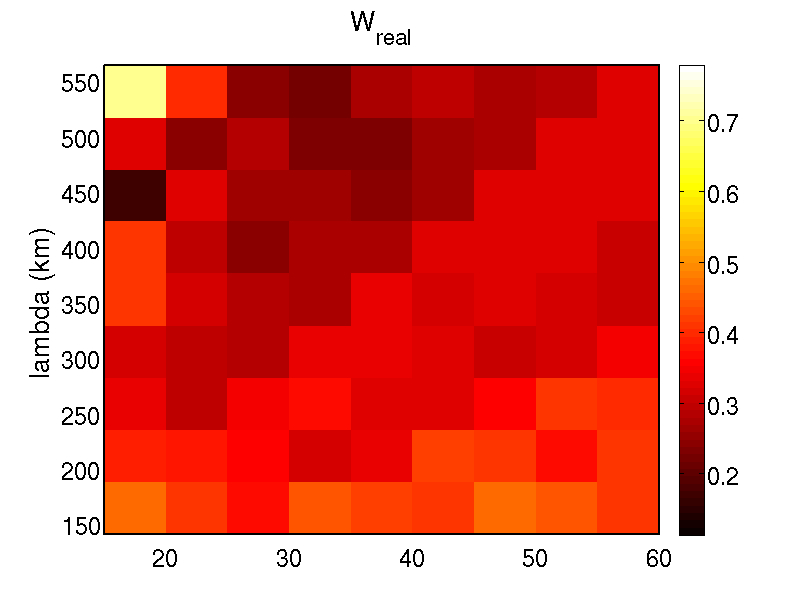
\includegraphics[width=0.4\linewidth]{scales_wM0Zauto_T15-5-60_Lauto}}
\subfigure[]{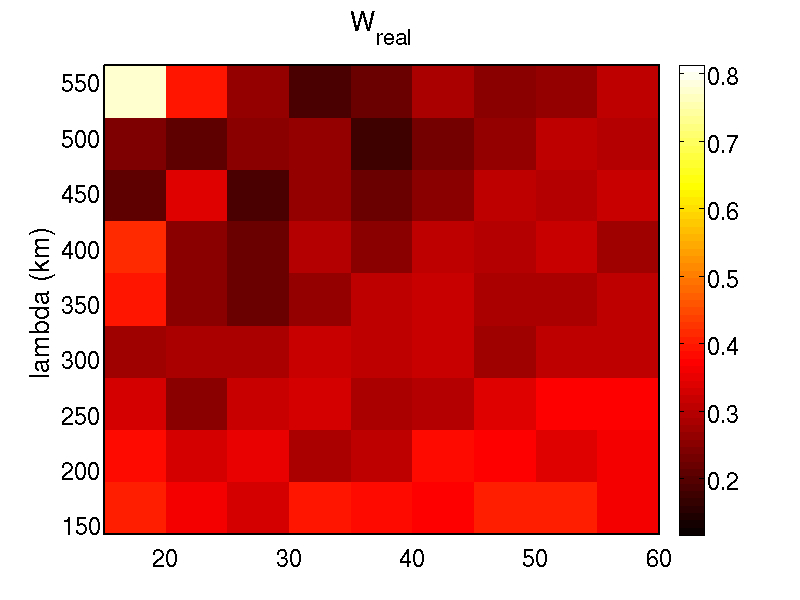
\includegraphics[width=0.4\linewidth]{scales_wauto_T15-5-60_Lauto}}
%\caption{{\footnotesize Modèle de vent NRLMSISE-00 à 01H00 UT. Vent zonal (a) et vent méridien (b). Les courbes pleines sont les profils aux coordonnées géographiques [0°N; 85°E] (utilisés pour les simulations numériques), les lignes en pointillés montrent les variations des valeurs dans une grille de coordonnées [$\pm$12°N; (75°E,95°E)].}}
\end{figure}
\end{frame}

\begin{frame}
\frametitle{le rôle du gradient de vent moyen}
% reprendre l'exemple du rapport
%TODO figures : amplification avec plusieurs valeurs de gradient vs plusieurs gammes de fréquences
\begin{figure}[!ht]
\centering
\subfigure[]{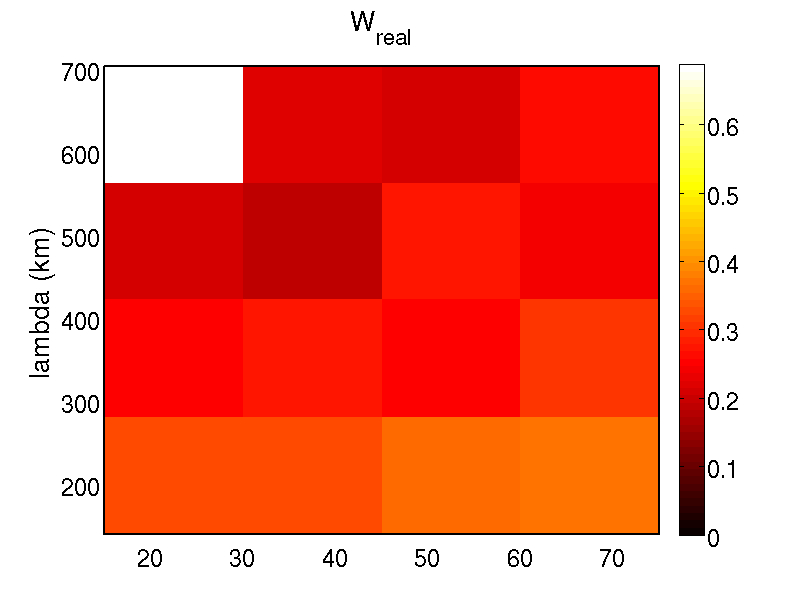
\includegraphics[width=0.3\linewidth]{scales_w0-20_T15-15-75_Lauto}}
\subfigure[]{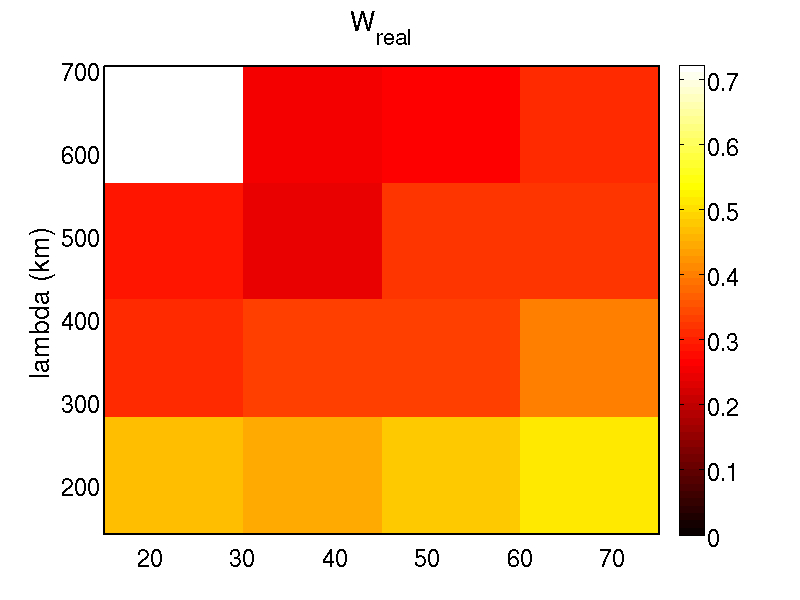
\includegraphics[width=0.3\linewidth]{scales_w0-50_T15-15-75_Lauto}}
\subfigure[]{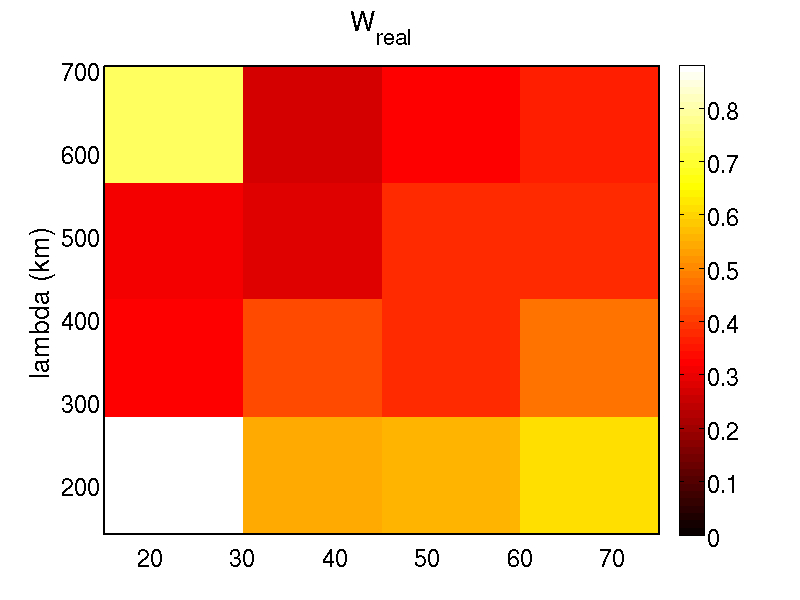
\includegraphics[width=0.3\linewidth]{scales_w0-75_T15-15-75_Lauto}}\\
\subfigure[]{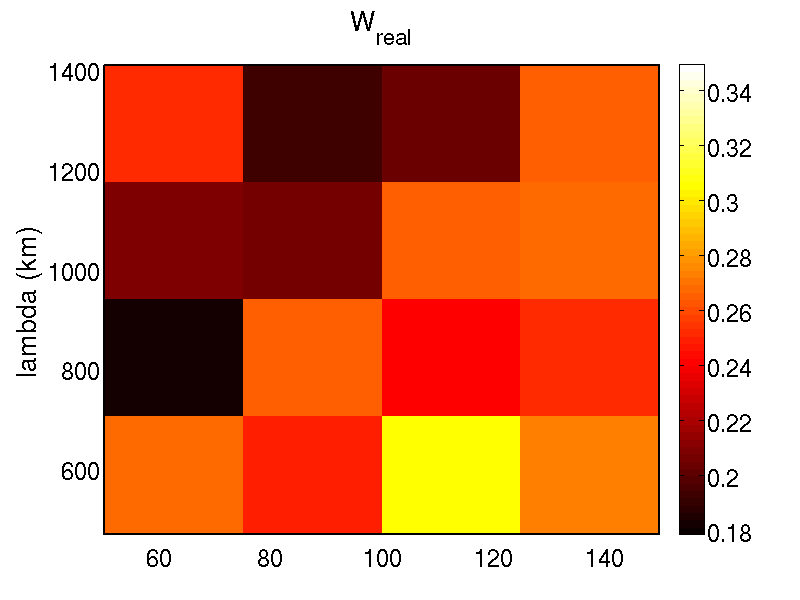
\includegraphics[width=0.3\linewidth]{scales_w0-20_T50-25-150_Lauto}}
\subfigure[]{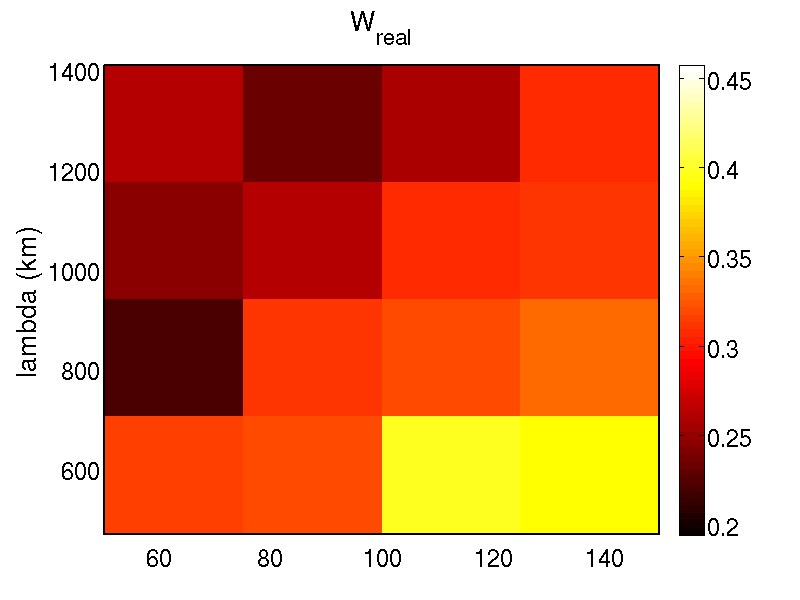
\includegraphics[width=0.3\linewidth]{scales_w0-50_T50-25-150_Lauto}}
\subfigure[]{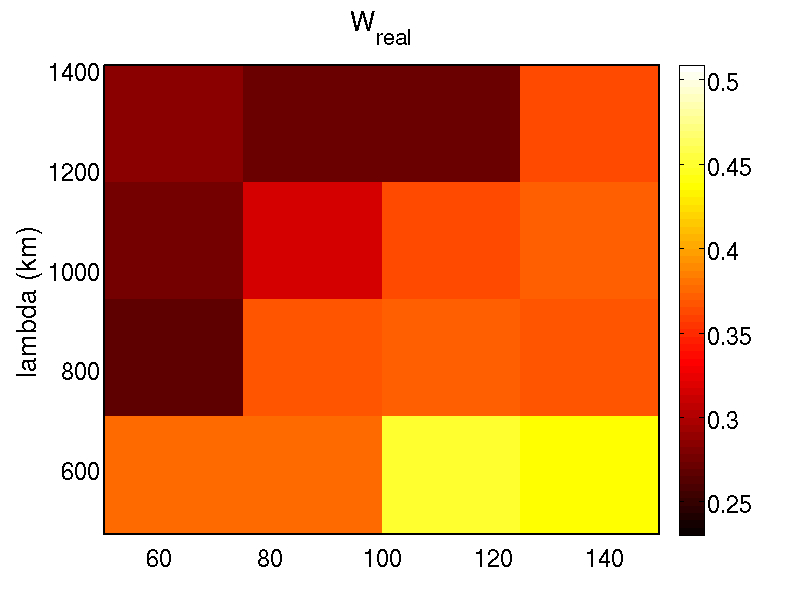
\includegraphics[width=0.3\linewidth]{scales_w0-75_T50-25-150_Lauto}}
%\caption{{\footnotesize Modèle de vent NRLMSISE-00 à 01H00 UT. Vent zonal (a) et vent méridien (b). Les courbes pleines sont les profils aux coordonnées géographiques [0°N; 85°E] (utilisés pour les simulations numériques), les lignes en pointillés montrent les variations des valeurs dans une grille de coordonnées [$\pm$12°N; (75°E,95°E)].}}
\end{figure}
\end{frame}

% -----------------------------
\section{effet de la viscosité}

\subsection{le modèle physique}

\begin{frame}
\frametitle{rôle de la diffusion de quantité de mouvement}
%TODO effet attendu, à partir de quelle altitude, etc.
\begin{minipage}{0.5\textwidth}
\begin{flushleft}
    Plusieurs phénomènes dissipatifs interviennent au cours de la propagation (viscosité, flux de chaleur, interactions d'onde).\\
    Viscosité faible de l'air ($\simeq 10^{-5}$) mais effet non négligeable lorsque la densité devient très faible.\\
\end{flushleft}
\end{minipage}
\begin{minipage}{0.5\textwidth}
\begin{flushright}
    \begin{figure}[!ht]
        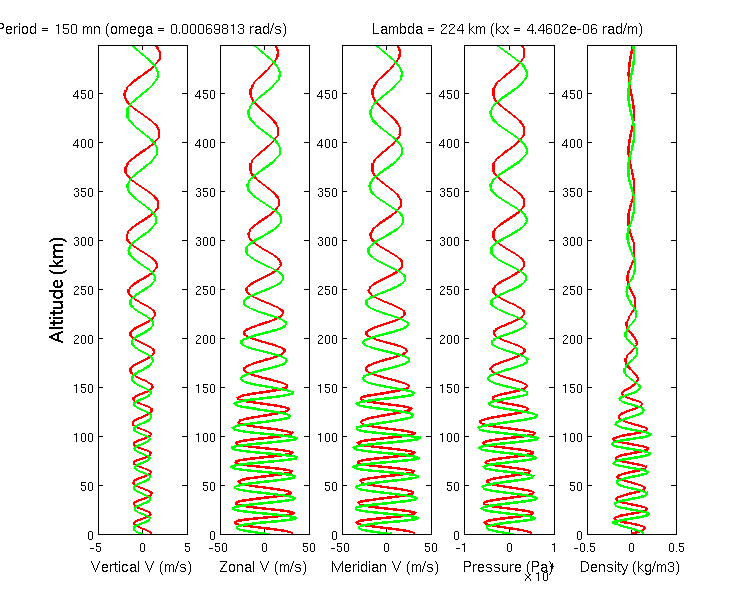
\includegraphics[width=\linewidth]{modes}
    \end{figure}
\end{flushright}
\end{minipage}
\end{frame}

\begin{frame}
\frametitle{rhéologie du système étudié}
\begin{align}
\rho \dt{v_i}
& = \deli{\jaune{\Tctrij}}{x_j} + \rho g_i \notag \\
& = \divergence \jaune{\Tctrdev} + \divergence \underbrace{(- \pression + \viscbulk \divergence \vv)}_{\jaune{\Tctrmoy}} + \rho \vg \notag
\intertext{et comme $G = 0$ pour les fluides, la \bleu{partie déviatorique} est purement \bleu{visqueuse}}
  & = \deli{2 \visc \Ttxdefijdev}{x_j} + \gradient \lp - \pression + \viscbulk \divergence \vv \rp + \rho \vg \notag
\end{align}
On montre que $2 \visc \divergence \Ttxdefdev = \visc \laplacien \vv$ (à $\visc$ constante !). De ce fait
\pifpaf{$\rho \dt \vv = \visc \laplacien \vv + \gradient \lp - \pression + \viscbulk \divergence \vv \rp + \rho \vg$}
\end{frame}

\subsection{vers l'implémentation numérique}

\begin{frame}
\frametitle{adimensionnement}
\begin{align}
u    & = U u^*, v = V v^*, w = W w^* \textrm{~avec~} U = V = W \notag \\
x    & = L x^*, y = L y^*, z = L z^* \notag \\
t    & = \frac{L}{U} t^*, P = \rho U^2 P^*, \rho = R \rho^* \notag
\end{align}
\begin{subnumcases}{}
    \deltet{\vv^*} + \lp \vv^* \cdot \gradient \rp \vv^* & $= -\gradient P^* + \frac{\mu}{\rho U L} \laplacien \vv^*$ \notag \\
    \divergence \vv^* & $= 0$ \notag \\
    \deltet{\rho^*} + \divergence \lp \rho^* \vv^* \rp & $= 0$ \notag
\end{subnumcases}\plop
Nombre de Reynolds : $Re = \Reynolds$\plop
Le système des perturbations doit être adimensionné ainsi.
\end{frame}

%\begin{frame}
%\frametitle{préconditionnement}
%\end{frame}

% ----------------
\section{}
\subsection{}

\begin{frame}
\frametitle{Perspectives}
\begin{itemize}
    \item terminer le code adimensionnel : coupler avec les vents, équation d'état
    \item passer du propagateur pseudo-spectral (étude modale) à une résolution par relation de dispersion
    \item passer en spectral complet (T.F.) : code 3D
    \item problème inverse à partir de sa signature atmosphérique : le séisme de Sumatra-Andaman
    \item paralléliser le code ?
\end{itemize}
\end{frame}

\end{document}

